\section{Evaluation}
\label{sec:evaluation}
How are we checking the validity of the goodness-criteria for splits? The examples below show that the algorithm captures the goodness criteria...
Data characteristics: what about cases where it splits crossing lines or the bullseye pattern?
Something about performance?

\subsection{Examples}
\subsubsection{Visual Patterns}
To illustrate the ability of our approach to pick out interesting Partitioners based on different visual patterns, we look at data about American universities and different Scagnostic measures. The Integrated Postsecondary Education Data System (IPEDS) is the primary source for data on colleges, universities, and technical and vocational postsecondary institutions in the United States via the National Center for Education Statistics.\footnote{\url{http://public.tableau.com/s/resources?qt-overview_resources=1}} We are interested in understanding the relationship between the percent of admitted students and the graduation rate of students with Bachelors degrees within $6$ years as in Figure~\ref{fig:original1}. 
\begin{figure}
 \centering 
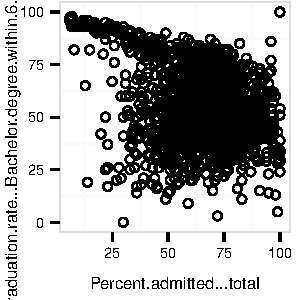
\includegraphics[width=2.25in,height=2.25in]{images/Percent_admitted_total-Graduation_rate_Bachelor_degree_within_6_years_total.pdf}
  \caption{Original interesting bivariate relationship}
 \label{fig:original1}
\end{figure}

\begin{figure}
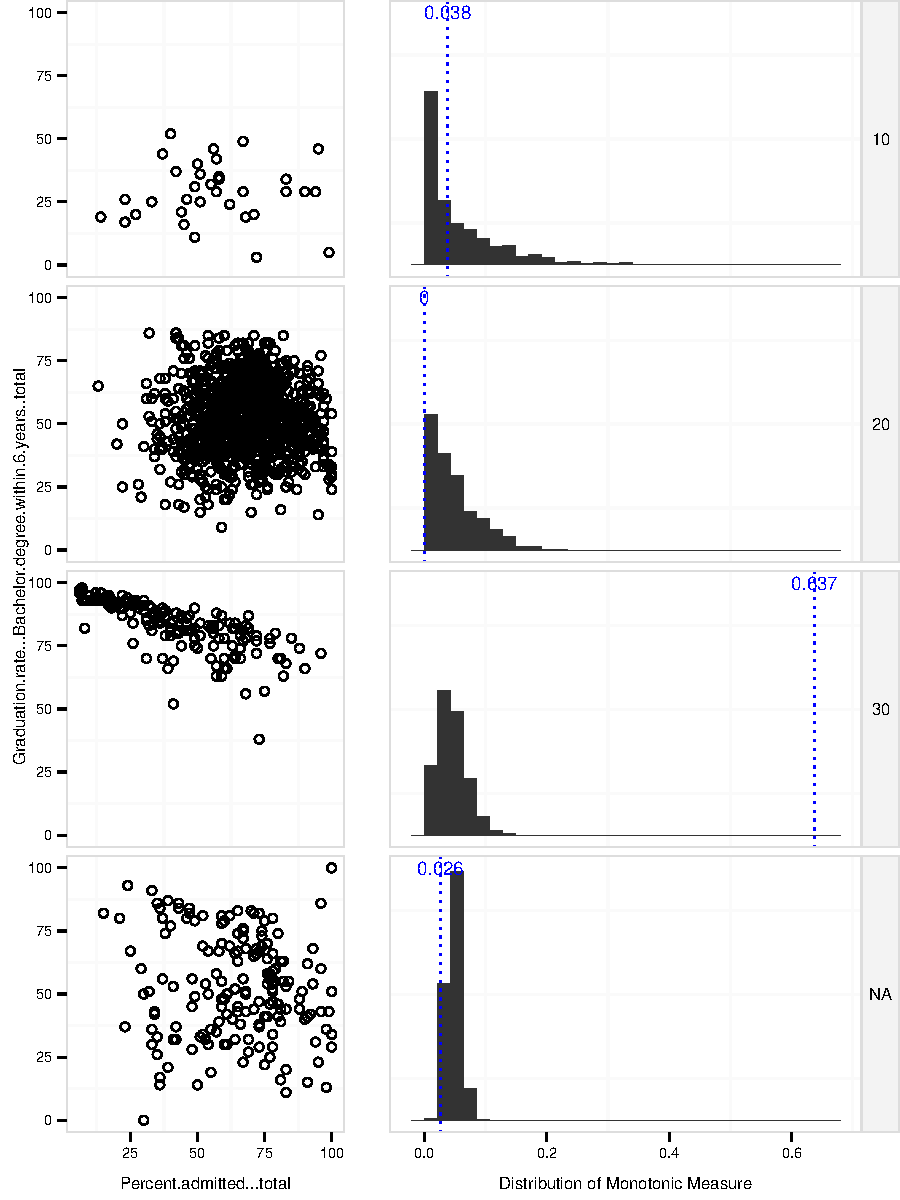
\includegraphics[width=3.5in,height=4in]{images/24_6604273087972-ACT_Composite_75th_percentile_score_bin.pdf}
  \caption{Monotonic}
 \label{fig:monotonic1}
\end{figure}

With the Monotonic Scagnostic as the measure to score splits, the highest ranked Partitioner is the variable labeled ACT\_Composite\_75th\_percentile\_score\_bin. This variable represents a disjoint, simple binning of the ACT Composite 75th percentile score into four categories, one of which is ``NA" - missing data code. Figure~\ref{fig:monotonic1} shows the resulting split with clearly interesting visual patterns in each facet of the resulting small multiple on the left. This Partitioner has succeeded in pulling apart revealing structure from the original bivariate relationship giving us a visual explanation of elements of the pattern in Figure~\ref{fig:original1}. 
The splits $\left\{{10, 20, 30, NA}\right\}$ have sizes $\left\{{36, 1010, 153, 335}\right\}$. Each histogram on the right shows the distribution of the Monotonic score on the bootstrapped samples of the same size as the facet it is aligned with on the left. The vertical, red, dashed line is a reference line for the score of the visual pattern in the left plot, so it can be visually compared to the reference distribution. In this case the strong Monotonic pattern in bin $30$ is a significant divergence from the expected range of values for the Monotonic score given the dataset and random samples without replacement of size $153$.

\begin{figure}
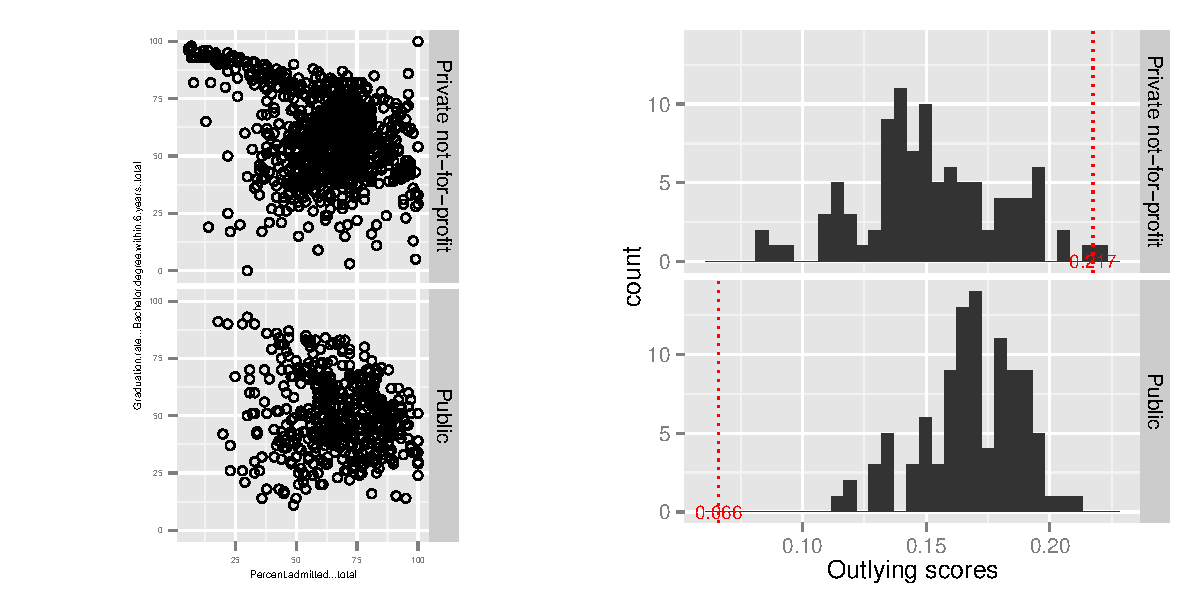
\includegraphics[width=3.5in,height=2.5in]{images/3_0003032851242-Control_of_institution.pdf}
  \caption{Outlying}
 \label{fig:outlying1}
\end{figure}

Selecting a different Scagnostic measure such as Outlying, ranks a different split as the most salient as seen in Figure~\ref{fig:outlying1}. Here, the Partitioner variable Control\_of\_institution produces a split that maximizes the z-score criterion over other variables despite not having a significant Outlying score on any facet as compared to the reference distributions seen on the right. The Outlying score considers the overall shape and density of the points in a two-dimensional point cloud so relatively evenly distributed sets of points will have low scores as seen in the distribution of the $563$ points for the ``Public" category in relation to the $971$ points in the ``Private not-for-profit" category.

\begin{figure}
 \centering 
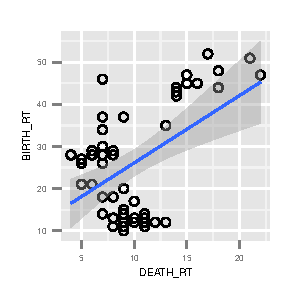
\includegraphics[width=2.25in,height=2.25in]{images/DEATH_RT-BIRTH_RT.pdf}
  \caption{Original interesting bivariate relationship}
 \label{fig:original2}
\end{figure}

\subsubsection{Divergence}
To examine the divergence criterion we investigate whether our approach can pick out ``confounding variates" such as those that cause Simpson's Paradox. The Ourworld dataset of UN statistics on world countries~\cite{Wilkinson2005GG,Wilkinson2008} has such a known relationship when considering the positive correlation between the variables Death\_Rate and Birth\_Rate as seen in Figure~\ref{fig:original2}. We seek to reveal the visual structure by conditioning on variables in the dataset. Of the six categorical variables in the dataset, the one with the largest score using the $R^2$ metric for the goodness of linear fit is the GNP seen in Figure~\ref{fig:r2}. This Partitioner variable pulls apart the group of points/countries negatively correlated in the ``D" category from the strongly positively correlated set of countries in the ``U" category. Also, we see that when we have a small number of points in a split (category $0$), the distribution of scores from random samples is wide and flat as it is easy to infer patterns with a few points but these have low support.

\begin{figure}
\raggedleft
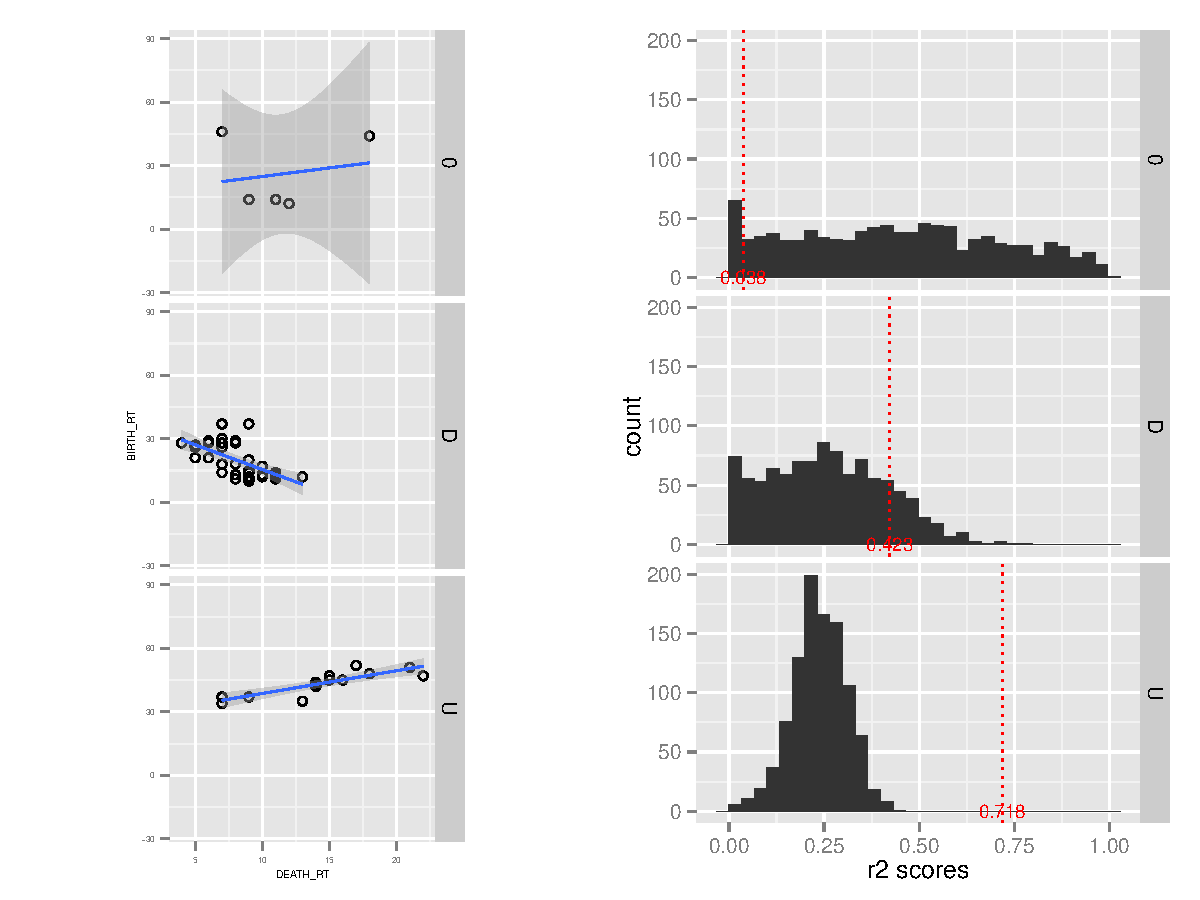
\includegraphics[width=3.5in,height=3.5in]{images/6_79024203387873-GNP.pdf}
  \caption{r2}
 \label{fig:r2}
\end{figure}

\subsubsection{Support}
We expect to be conservative in our assessment of interesting patterns for ones with low support or determined by a small number of points. We see this in another split of the Ourworld data from the earlier example. Figure~\ref{fig:r2-leader} shows another interesting conditioning of the original interesting bivariate relationship. The higher cardinality Partitioner variable ``Leader" produces small individual splits which can be seen to have wide score distributions. Also, the splits produced by ``Leader" are not highly significant except for the ``Marxist" category.

%Risk Factors Associated with Low Infant Birth Weight~\cite{Hosmer1989}
\begin{figure}
\raggedleft
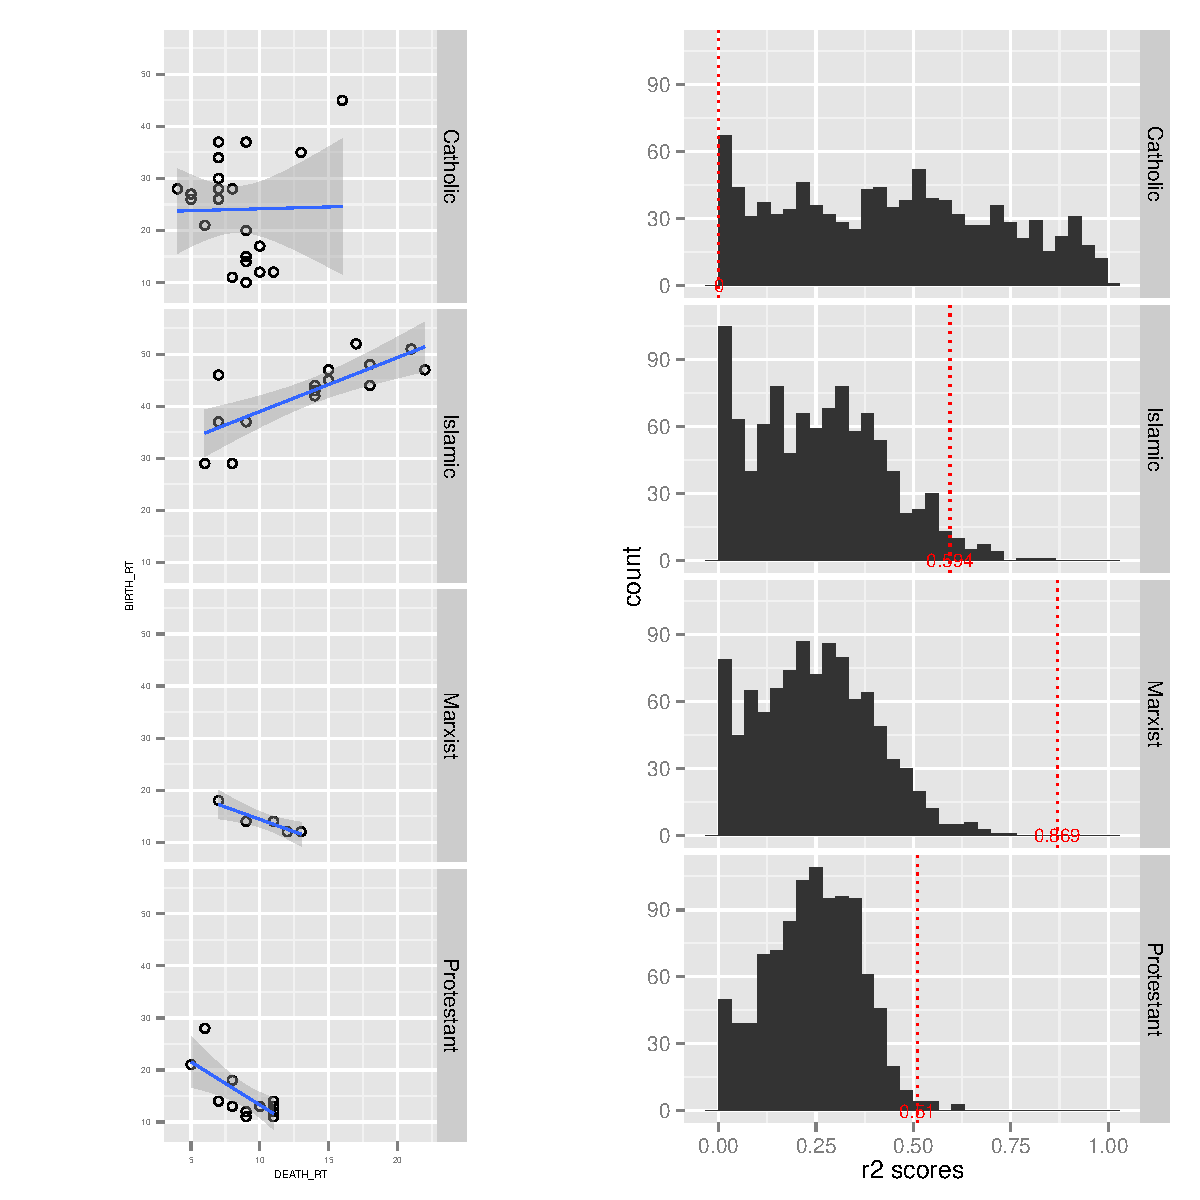
\includegraphics[width=3.5in,height=3.5in]{images/4_16075880239701-LEADER.pdf}
  \caption{r2}
 \label{fig:r2-leader}
\end{figure}

\subsubsection{Degrees of Freedom}
High-cardinality Partitioners create a large number splits, which likely produce splits with low support as the observations get distributed among more facets. Not happy with this SuperStore example...
\begin{figure}
 \centering 
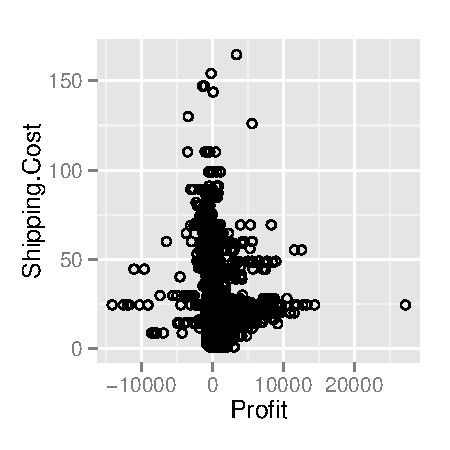
\includegraphics[width=2.25in,height=2.25in]{images/Profit-Shipping_Cost.pdf}
  \caption{Original interesting bivariate relationship}
 \label{fig:original3}
\end{figure}

\begin{figure}
\raggedleft
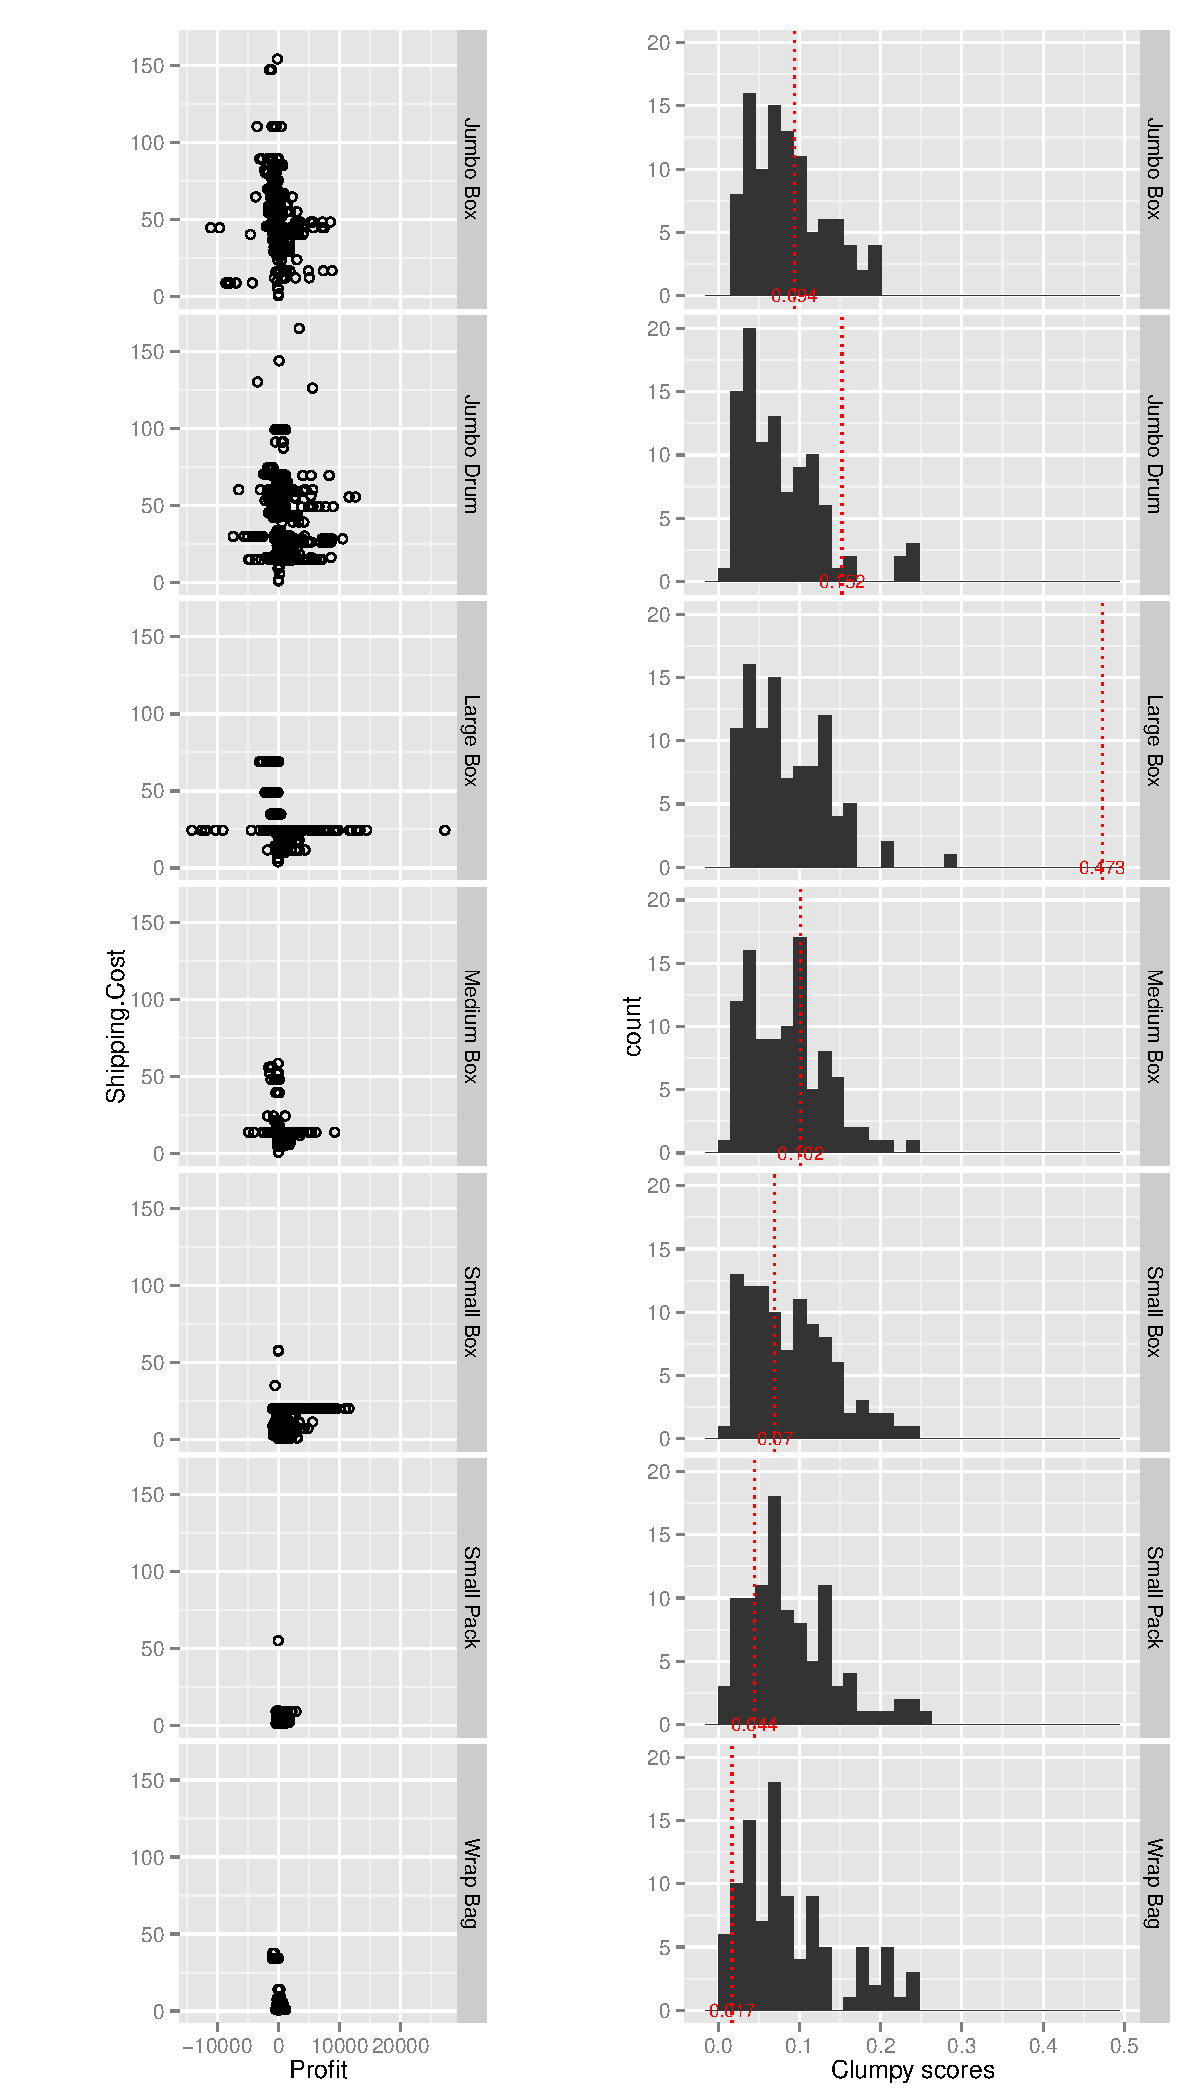
\includegraphics[width=3.5in,height=4in]{images/7_64436895673431-Product_Container.pdf}
  \caption{r2}
 \label{fig:r2}
\end{figure}

\begin{figure}
\raggedleft
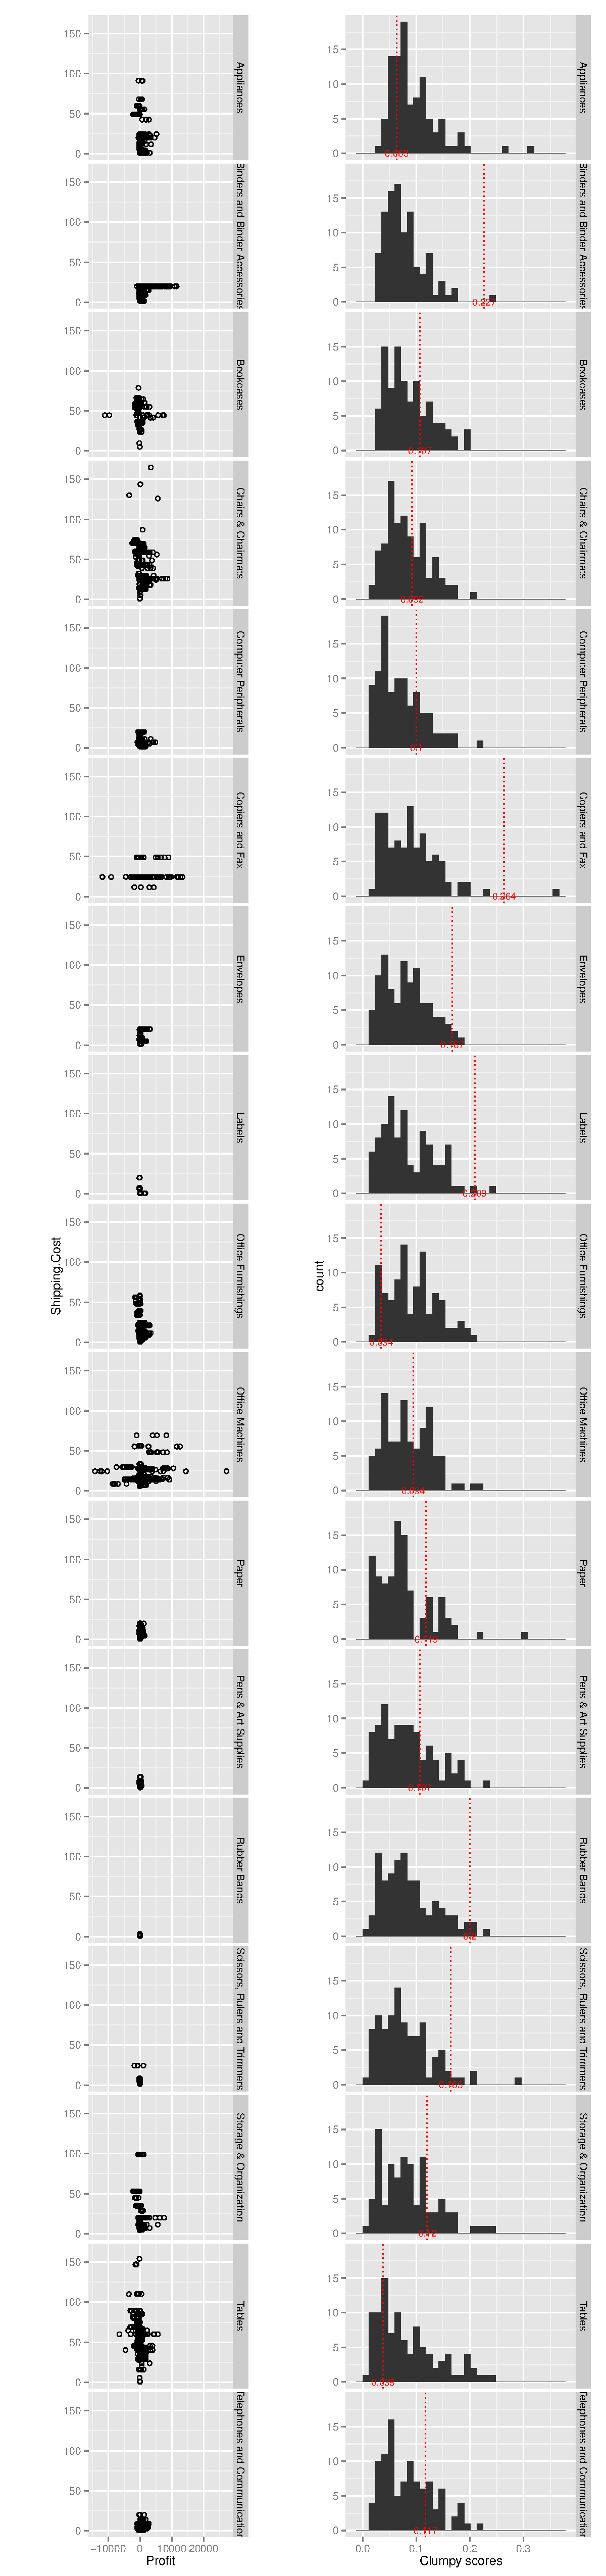
\includegraphics[width=3.5in,height=8in]{images/3_67472603496804-Product_Sub_Category.pdf}
  \caption{r2}
 \label{fig:r2}
\end{figure}


\section{Discussion}
\label{sec:discussion}
Our approach of selecting Partitioner variables that showcase interesting visual explanations is generalizable in terms of allowing for a diversity of measures used to capture ``interesting visual structure". The wide range of measures surveyed~\cite{Bertini2011} can be used w/ our method based on the plot type of interest to describe the visual pattern of interest to find when partitioning a view.

Furthermore, we can use this approach of selecting good splits of a data view to guide other multivariate exploratory data analysis applications.

Decision tree approach of guided EDA.

Trellis displays present a grid of plots of the same type showing the same variables conditioned on a Partitioner variable that determines the subsets of points shown in each plot. These displays are a very useful multivariate display as they are simple to interpret and provide an overview of large datasets for exploratory data analysis. Crucial to the layout of small multiples is the selection of a Partitioner variable to specify faceting into plots by rows and/or columns. This choice can then be repeated to facet the resulting plots further applying crossing and nesting.


